\documentclass[letterpaper]{article} % DO NOT CHANGE THIS
% AAAI-27 Author Kit (official, https://aaai.org/authorkit27/, AuthorKit27.zip, aaai2027.sty dated 2026-10-21).
% Anonymous-submission mode; author information is a placeholder pending the user's decision.
\usepackage[submission]{aaai2027}  % DO NOT CHANGE THIS
\usepackage[hyphens]{url}  % DO NOT CHANGE THIS
\usepackage{graphicx} % DO NOT CHANGE THIS
\urlstyle{rm} % DO NOT CHANGE THIS
\def\UrlFont{\rm}  % DO NOT CHANGE THIS
\usepackage{natbib}  % DO NOT CHANGE THIS AND DO NOT ADD ANY OPTIONS TO IT
\usepackage{caption} % DO NOT CHANGE THIS AND DO NOT ADD ANY OPTIONS TO IT
\frenchspacing  % DO NOT CHANGE THIS
\usepackage{algorithm}
\usepackage{algorithmic}
\usepackage{booktabs}
\usepackage{array}
\usepackage{amsmath}
\usepackage{placeins} % \FloatBarrier keeps appendix floats in their sections
\pdfinfo{
/TemplateVersion (2027.1)
}
\setcounter{secnumdepth}{2} % Section numbers enabled (permitted by the template: 0, 1 or 2).

\title{BrickMore}
% TODO 待用户确认: title is unchanged from V1.3; AAAI asks for a descriptive mixed-case title.
\author{
    % TODO 待用户确认: author names and affiliations are placeholders until the user provides them.
    Author Name(s) to Be Added\textsuperscript{\rm 1}
}
\affiliations{
    \textsuperscript{\rm 1}Affiliation(s) to Be Added\\
    email@to-be-added
}

\begin{document}

\maketitle

\begin{abstract}
Generating brick structures from text is a geometric assembly problem: a layout must match a natural-language description while placing discrete pieces that fit in a bounded grid, connect through studs, and form one consistent structure. We present BrickMore, a text-to-brick framework that combines agentic batch generation of training data, language-model fine-tuning, and post-generation geometric repair in order to learn and constrain a spatial representation of brick assemblies. Using GPT-6.1 Sol, we run an agentic batch-generation pipeline in which the model writes parametric generator programs that then emit three-dimensional voxel models in batches. The resulting BrickMore-48 source dataset contains 80,000 voxel models across 21 object categories on a $48^3$ grid, each with five bilingual captions at different levels of detail (400,000 records). Same-color tiling, connectivity analysis, and local bridging and retiling convert the shapes into brick layouts; in the latest integrated release, 79,301 models pass the specified geometric checks. We fine-tune Qwen3-1.7B with low-rank adaptation (LoRA) on English captions and brick-placement sequences so that it predicts brick dimensions and positions from text. After generation, the pipeline forms a voxel union from the in-bounds portions of supported placements, uses mixed-integer linear programming (MILP) to seek an exact cover, and checks for a single stud-connected component. On 114 shared prompts and under a common rendering protocol, the evaluated BrickMore outputs (110 retiled, 4 raw) obtain the highest mean scores on three text--image alignment metrics, and a mean invalid-placement ratio of 0.00\%, matching BrickGPT.
\end{abstract}

\begin{figure*}[t]
\centering
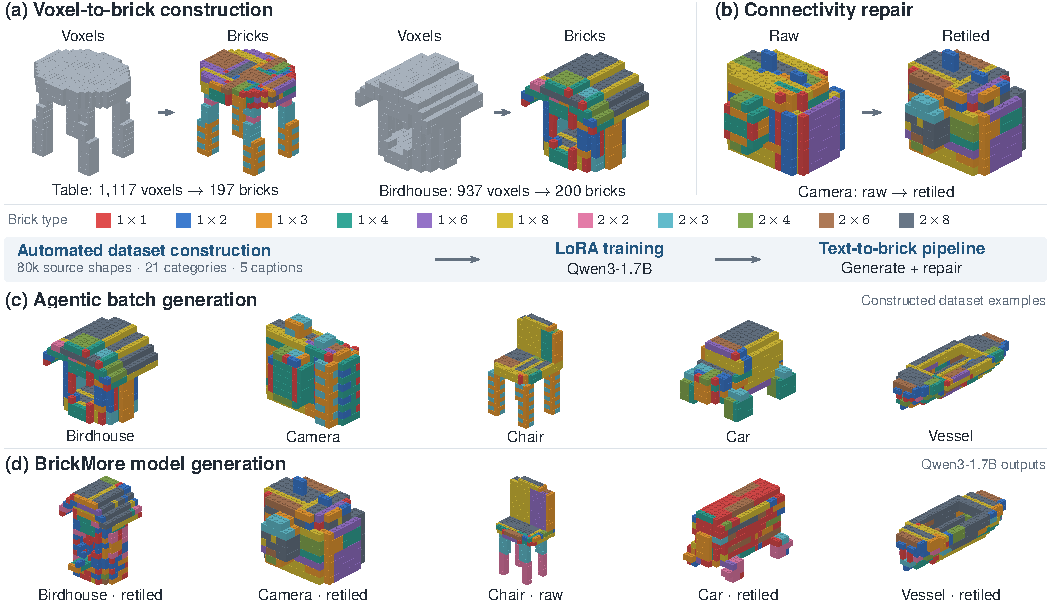
\includegraphics[width=0.94\textwidth]{figure1.pdf}
\caption{\textbf{BrickMore overview.} (a) Source voxels are converted into rectangular bricks. (b) Raw predictions are retiled to repair connectivity. (c) Examples from agentic batch generation of voxel data. (d) Outputs of the fine-tuned Qwen3-1.7B pipeline. Colors encode brick type independent of orientation; they are visualization labels, not predicted appearance. Voxels are shown in gray.}
\label{fig:teaser}
\end{figure*}

\section{Introduction}
Text-to-3D generation lets users describe and create objects in natural language~\cite{dreamfusion}. Generating brick structures adds the requirement that a target shape be represented as discrete pieces and their spatial placements. Beyond matching the text, the structure must avoid overlaps and keep the bricks connected: a layout may resemble the described object while containing intersecting bricks or disconnected parts. The setting is therefore one of geometric reasoning and object assembly, in which the system must decide how bricks fit, interlock, and remain connected in space, not only whether the overall shape resembles the described object.

Prior work has explored text-driven brick generation with different representations and constraints. BrickGPT trains an autoregressive language model on paired text and brick structures and applies validity checks and physics-aware rollback during inference~\cite{brickgpt}. BrickNet uses a graph-backed representation to generate assembly sequences over a broader range of parts and connection types~\cite{bricknet}. Both show that structural representations and generation-time constraints matter for brick modeling.

For voxel-based shapes, spatial adjacency between voxels does not imply a valid connection between bricks: a voxel shape can form one connected volume even when the bricks covering it only touch side by side without stud connections. This distinction affects both data construction and generation. Converting voxel shapes into training targets requires attention to coverage and stud connectivity, and predicted layouts may contain overlaps or disconnected components that require further processing.

We present BrickMore to study this problem. With GPT-6.1 Sol, we develop an agentic batch-generation pipeline: the model writes parametric generator programs, the programs emit voxel models in batches, and we convert the models into brick layouts. The source dataset contains 80,000 models across 21 categories on a $48^3$ grid, each with five bilingual captions. Occupied voxels are tiled with same-color rectangular bricks, and connection analysis with local bridging and retiling addresses ungrounded components; limited changes to the source voxels are recorded separately. In the latest integrated release, 79,301 models pass the specified geometric checks.

We fine-tune Qwen3-1.7B~\cite{qwen3} with LoRA~\cite{lora} on English captions and brick-placement sequences. Given a prompt, the model predicts brick dimensions and positions; the current output does not include color. To handle overlaps and connectivity defects, we form a target union from the in-bounds voxels of supported placements, use MILP to seek an exact cover, and check for a single stud-connected component; when no cover is found within the solver budget, a new sampling seed can be queued. The $48^3$ workspace, multi-level captions, and fixed spatial serialization define what the model learns, while conversion-time checks and post-generation exact-cover retiling constrain coverage, overlaps, and stud connectivity. The connectivity check is geometric; physical stability and assembly-order feasibility require separate evaluation.

We compare the provided outputs of BrickMore, BrickGPT, and BrickNet on 114 shared prompts spanning 21 categories and five description levels, measuring text--image alignment with VQAScore, PE, and SigLIP2 and the invalid-placement ratio $P_{\mathrm{inv}}$. Under a common rendering protocol, BrickMore has the highest mean on all three alignment metrics, and BrickMore and BrickGPT both have a mean $P_{\mathrm{inv}}$ of 0.00\% in exported file order. These results describe the provided outputs under the stated protocol and do not by themselves establish physical stability or assembly feasibility.

Our contributions are as follows.
\begin{enumerate}
\item An automated $48^3$ voxel data-generation pipeline based on agentic batch generation with GPT-6.1 Sol, which writes parametric generator programs that produce 80,000 source models across 21 categories with five bilingual captions each; 79,301 models pass the specified geometric checks in the latest integrated release. The data supply geometrically checked layouts for fine-tuning a text-conditioned spatial representation of brick assemblies.
\item A voxel-to-brick conversion pipeline that combines same-color tiling, connection analysis, and local bridging and retiling, and records limited changes to source voxels, so that training targets encode stud-connected assemblies rather than voxel adjacency alone.
\item A fine-tuned Qwen3-1.7B text-to-brick generator combined with post-generation repair based on voxel unions, exact-cover MILP, and connectivity checks.
\end{enumerate}


\begin{figure*}[t]
\centering
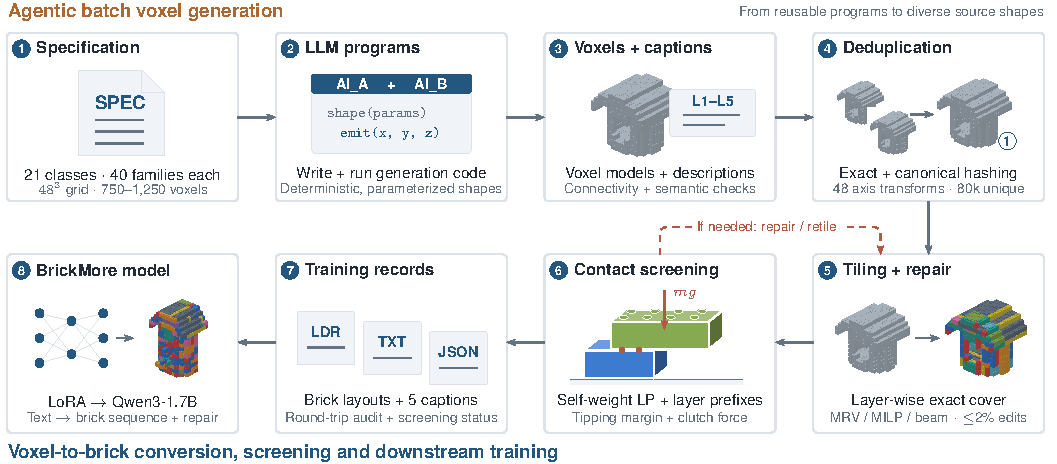
\includegraphics[width=0.94\textwidth]{figure2.pdf}
\caption{\textbf{Data-construction workflow.} Parametric programs written by GPT-6.1 Sol through agentic batch generation produce voxel shapes and captions, followed by deduplication, voxel-to-brick tiling, repair, contact-based screening, and audited export for fine-tuning. The dashed arrow denotes repair or retiling when needed. Screening is distinct from a guarantee of physical stability. Brick colors follow the legend in Figure~\ref{fig:teaser}.}
\label{fig:data-workflow}
\end{figure*}

\section{Related Work}
\paragraph{Brick assembly and generation.}
Learning-based brick construction has been studied as graph generation~\cite{thompson2020lego}, as combinatorial construction with deep reinforcement learning~\cite{brickbybrick}, and as interactive structural understanding in a LEGO simulator~\cite{breakandmake}. For text-conditioned generation, BrickGPT represents a design as an autoregressively generated sequence of brick placements and uses brick-level rejection sampling with physics-aware rollback at inference~\cite{brickgpt}; BrickNet represents part connectivity through a graph-backed parametrization and trains autoregressive models on its assembly sequences~\cite{bricknet}. BrickMore also generates placement sequences from text, on a larger $48^3$ grid with a 20-type library, and examines geometric reconstruction and connectivity in a separate post-generation stage.

\paragraph{Stability analysis.}
StableLego analyzes the structural stability of block-stacking assemblies with a force-balance optimization~\cite{stablelego}. Such analyses depend on their mechanical assumptions. In BrickMore, geometric connectivity and the contact-based screening in the dataset materials address different properties; neither alone establishes that every generated model can be physically assembled and remains stable.

\paragraph{Procedural data and parameter-efficient fine-tuning.}
Procedural generation is a common way to obtain large, controllable 3D training data~\cite{infinigen}. BrickMore uses a language model to write the procedural generators rather than to emit coordinates directly. The generator itself is adapted with LoRA~\cite{lora}, following the BrickGPT recipe of fine-tuning a pretrained language model on serialized brick sequences~\cite{brickgpt}.

\section{Dataset Construction}
\label{sec:dataset}
\subsection{Parametric Voxel Generation}
BrickMore-48 contains 80,000 voxel models on a $48^3$ grid across 21 categories (3,805--3,810 per category), each paired with five bilingual captions at levels L1 (concise) to L5 (detailed). The models are produced by parametric generator programs written through agentic batch generation with GPT-6.1 Sol; the programs, rather than the language model itself, emit the voxel coordinates. Each record includes a geometry plan and a dataset version identifier for reproduction, and exact and canonical (48 axis/sign transforms) occupancy hashes show no duplicates across the two 40,000-model shards. Figure~\ref{fig:data-workflow} summarizes the workflow; sample shapes are shown in Appendix~\ref{app:dataset}.


\subsection{Voxel-to-Brick Conversion and Checks}
The conversion pipeline tiles occupied voxels with same-color rectangular bricks and analyzes their connections. Local bridging and retiling address ungrounded components, and changes to source voxels are recorded separately. Each converted model carries a \texttt{validation.json} that records three geometric constraints: the occupied voxels form a single six-neighbour connected component, every brick component is grounded, and the bricks exactly cover the (derived) target voxels. Under these release rules a layout may consist of several brick components that are each grounded; this criterion differs from the single stud-connected component enforced by post-generation retiling (Section~\ref{sec:model}). The dataset materials also describe a contact-based gravity screening procedure; its outputs are screening results under stated assumptions rather than proof of physical stability (Appendix~\ref{app:dataset}); training-data selection uses the geometric checks.

\subsection{Integrated Release and Training Corpus}
The full retile release records 79,298 geometrically passing models; the 702 failures (0.88\%) are concentrated in table (132), bookshelf (110), vessel (89), bowl (79), and bus (75). Replacing all 1,905 batch-B piano slots (1,902 passing) with a regenerated release in which all 1,905 pass gives an integrated count of $79{,}298-1{,}902+1{,}905=79{,}301$ passing models. This number is computed from the two release reports, not from a new full-dataset verification run, and the original A/B download does not apply the replacement automatically. Fine-tuning uses only geometrically passing models (Table~\ref{tab:training-data}).

\begin{table}[t]
\centering
\small
\setlength{\tabcolsep}{4pt}
\begin{tabular}{lr}
\toprule
Item & Count \\
\midrule
Source models / categories / grid & 80,000 / 21 / $48^3$ \\
Bilingual caption records & 400,000 \\
Failing in full retile release & 702 (0.88\%) \\
Passing in full retile release & 79,298 \\
Piano models restored by revised release & 3 \\
Integrated passing models & 79,301 \\
(model, English caption) samples & 396,610 \\ % TODO verify sample count (待用户确认)
Training / validation samples & 356,955 / 39,655 \\
Tokens over 3 epochs & 2,228,044,818 \\ % TODO verify token count (待用户确认; model card says ~2.19B)
\bottomrule
\end{tabular}
\caption{Dataset and fine-tuning corpus.}
\label{tab:training-data}
\end{table}
% TODO verify sample count (待用户确认)
% 79,301 models x 5 captions = 396,505, which differs from the reported 396,610 by 105.
% A released model card states "79,322 models x 5 captions = 396,610 samples" and "~2.19B tokens total";
% these conflict with the 79,301 integrated count and with 2,228,044,818 tokens.
% trainer_state.json / build_stats.json were not found. Do not resolve without user confirmation.

\section{BrickMore Text-to-Brick Model}
\label{sec:model}
\subsection{Fine-Tuning}
\label{sec:training}
We fine-tune Qwen3-1.7B on BrickMore-48 with a library of 20 brick types. Relative to StableText2Brick used by BrickGPT ($20^3$, 14 types), the library adds six footprints ($3{\times}2$, $2{\times}3$, $3{\times}1$, $1{\times}3$, $2{\times}8$, $8{\times}2$). Each object occupies 750--1,250 voxels with coordinates in $\{0,\ldots,47\}$. Training uses only the English captions (\texttt{captionEn}, L1--L5); the Chinese captions are not used. Samples are split by model at a 9:1 ratio, so the captions of one model never straddle the split.

Each sample is a three-turn chat, structurally identical to the official BrickGPT data-preparation script: a system prompt (``You are a helpful assistant.''), a user instruction adapted to the $48^3$ world that lists the 20 allowed dimensions, and an assistant reply with one brick per line, e.g.\ $2{\times}4\ (x,y,z)$. No thinking content is used; inference sets \texttt{enable\_thinking=False} to match training. Brick dimensions are serialized Y-first, then X, which differs from the StableText2Brick convention; training and inference share this convention, and downstream parsers must restore the orientation consistently.

Hyperparameters follow the Qwen3 fine-tuning script in the official BrickGPT repository (Table~\ref{tab:finetune-config}) rather than the LLaMA numbers in the original paper; Appendix~\ref{app:training} compares the two. Sequences are unpacked so that each caption--sequence boundary is preserved, and dependencies are pinned to the official TRL~0.17 stack. Training runs 133,860 steps in 25.3 hours ($\approx$202 GPU-hours). Validation loss, computed every 500 steps on a 2,000-sample validation subset, reaches its minimum of 0.0308 at step 79,000 (epoch 1.77) and rises to 0.0339 by the end of epoch 3. Because \texttt{load\_best\_model\_at\_end} is enabled, the released weights are those of step 79,000, so the additional third epoch does not degrade the released model. Full loss curves are listed in Appendix~\ref{app:training}.

\begin{table}[t]
\centering
\small
\setlength{\tabcolsep}{3pt}
\begin{tabular}{@{}l>{\raggedright\arraybackslash}p{0.58\linewidth}@{}}
\toprule
Item & Value \\
\midrule
Base model & Qwen3-1.7B (bf16) \\
Adaptation & LoRA, $r=16$, $\alpha=32$, dropout $0.05$, all linear layers \\
Optimization & LR $10^{-4}$, cosine, 100 warm-up steps, 3 epochs \\
Batch / max length & effective 8 (8 GPUs $\times$ 1) / 8,192 \\
Hardware & DDP, 8$\times$RTX 4090D (24\,GB) \\
Released checkpoint & step 79,000 (best validation loss) \\
Software & transformers 4.51.3, trl 0.17.0, peft 0.15.2 \\
\bottomrule
\end{tabular}
\caption{Fine-tuning configuration (details in Appendix~\ref{app:training}).}
\label{tab:finetune-config}
\end{table}

\begin{figure*}[t]
\centering
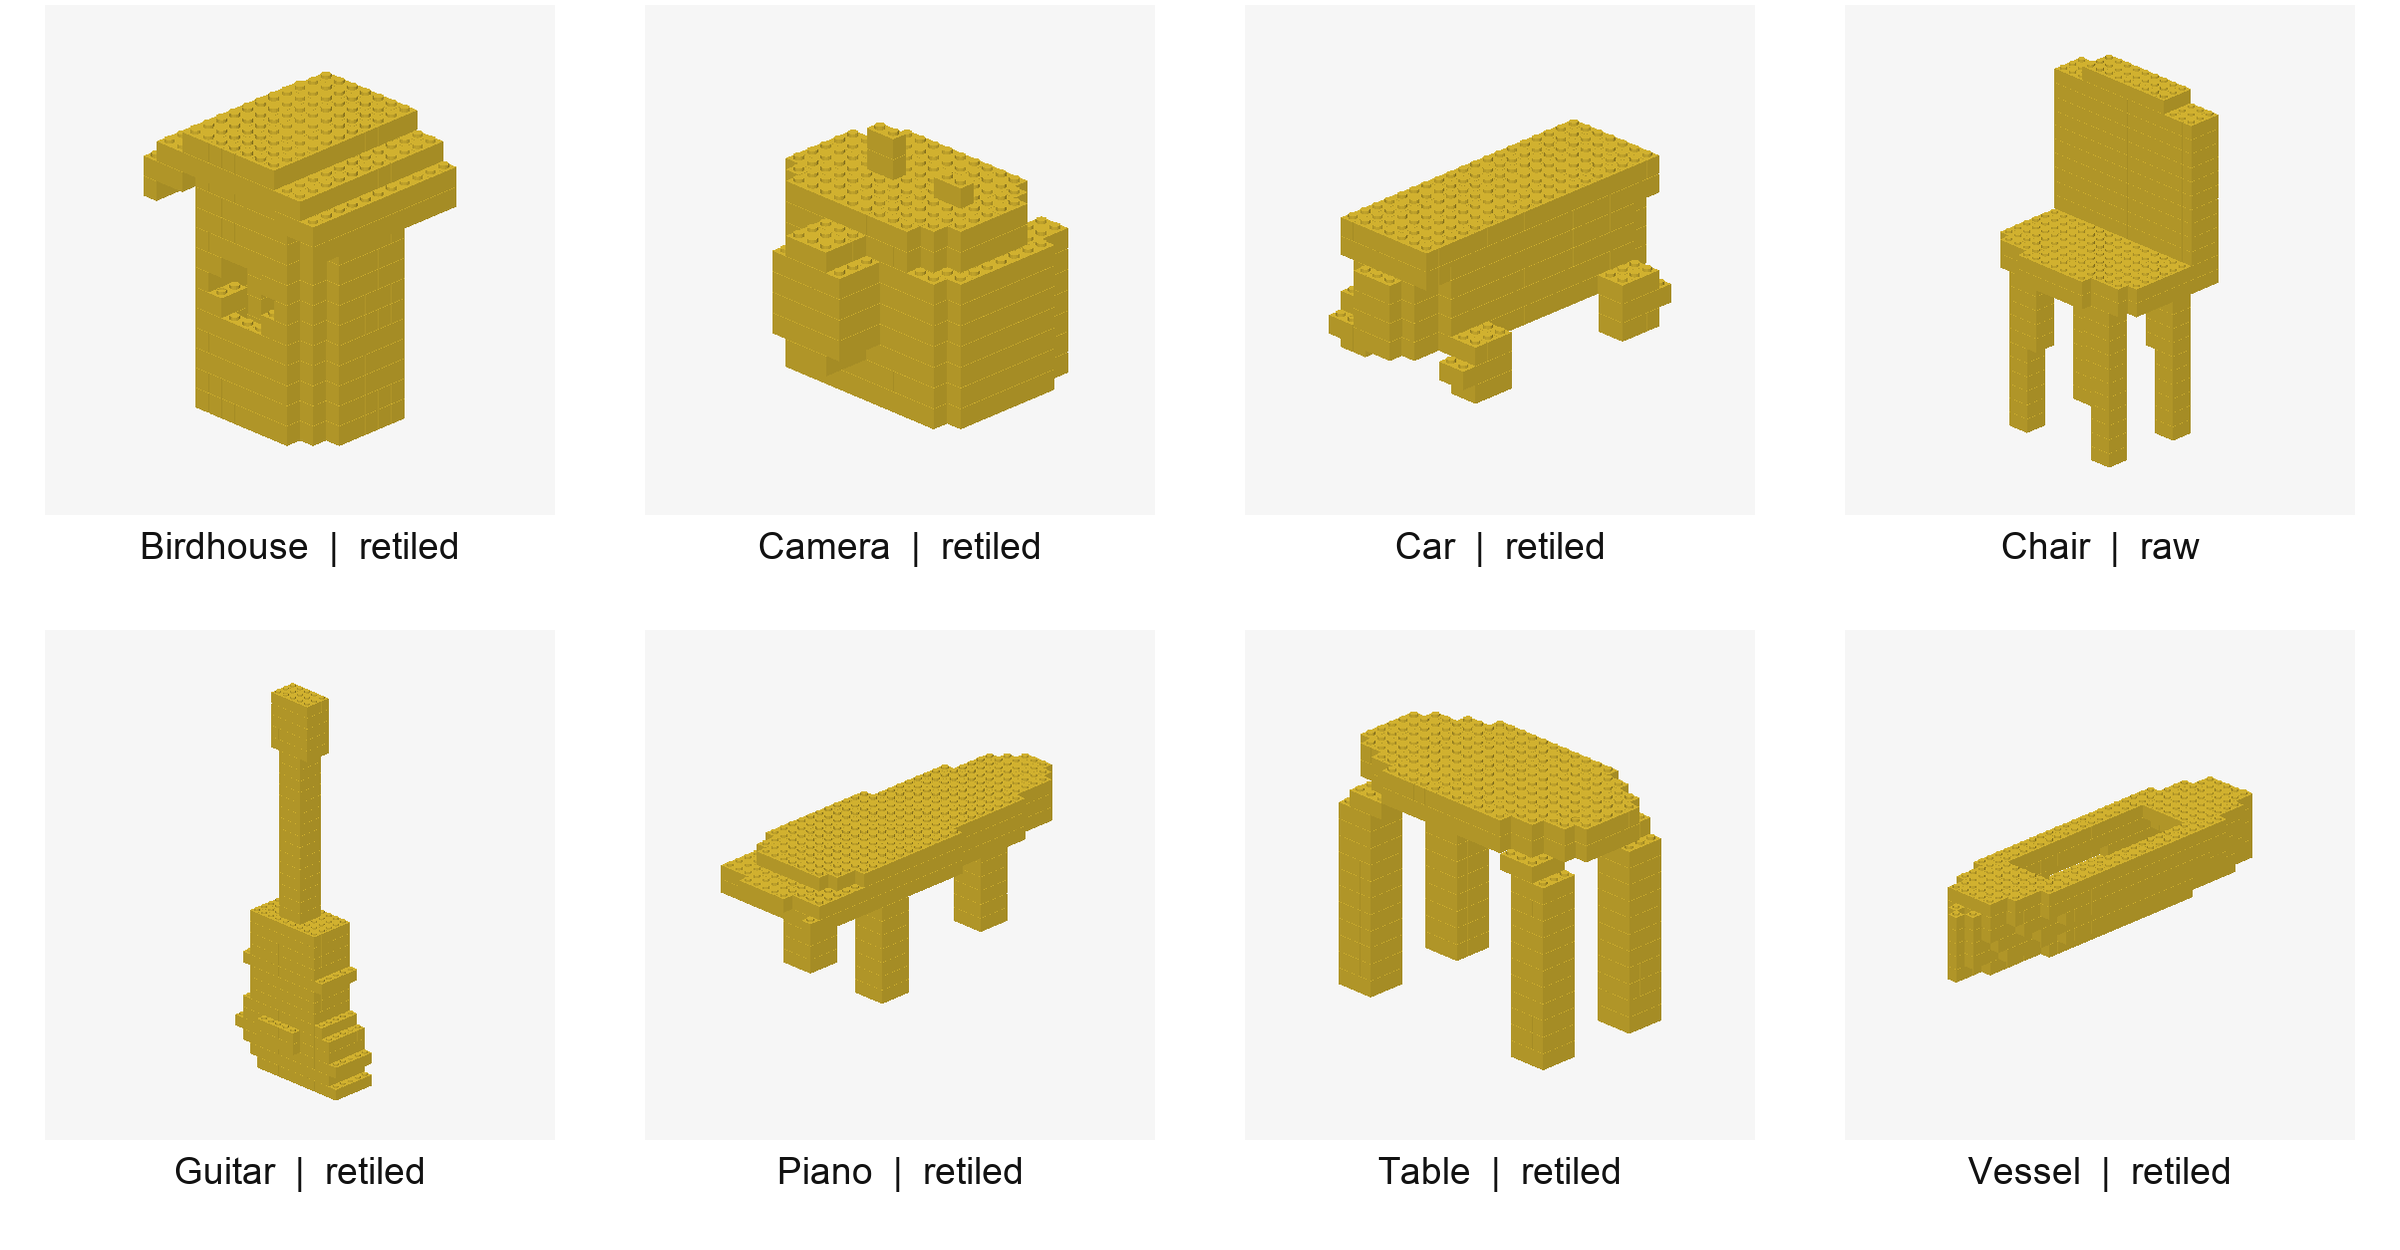
\includegraphics[width=0.75\textwidth]{figures/generated_gallery.png}
\caption{Selected BrickMore outputs from the 114-prompt evaluation, rendered with the uniform evaluation protocol (not photographs of physical assemblies). In this gallery, one chair is raw and the other outputs are retiled; in the full main comparison, 4 of the 114 BrickMore outputs are raw.}
\label{fig:gallery}
\end{figure*}

\subsection{Inference and Retiling}
Inference follows the seed-escalation and repair procedure in Algorithm~\ref{alg:inference-retiling}. The model samples a placement sequence with thinking disabled, temperature $0.7$, top-$p$ $0.9$, and at most $8192$ new tokens, using seeds $42$, $104$, and $2026$ in order. A candidate is accepted when generation completes (ends with an end-of-sequence token) and the geometry validator reports no errors. Otherwise, the pipeline keeps the completed draft with the fewest validator error records $\mathrm{Err}(\cdot)$ (line format, library membership, bounds, and overlaps). It then forms the voxel union $C$ of the in-bounds cells of supported library placements, solves a shape-preserving exact cover of $C$ with a single stud-connected component by MILP under a $12$--$60$--$180$\,s time ladder, and audits the result independently. If no cover is found within this budget, the raw draft is retained and a new seed may be queued. A separate recovery path may extend the budget to $600$\,s and sample seeds outside $S$; it is not part of the default loop. We call the MILP output the \emph{retiled} layout (files are named \texttt{stitched}) and the model's draft the \emph{raw} layout.

\begin{algorithm}[t]
\caption{BrickMore inference and retiling}
\label{alg:inference-retiling}
\small
\begin{algorithmic}[1]
\REQUIRE prompt $c$; fine-tuned model $\theta$; library $\mathcal{L}$ (20 types); seeds $S=(42,104,2026)$; MILP tiers $T=(12,60,180)$\,s
\ENSURE $(B_{\mathrm{out}}, \textit{status})$, $\textit{status}\in\{\textsc{Success},\textsc{Draft},\textsc{Failed}\}$
\STATE $B \gets \emptyset$; $A \gets \emptyset$
\FOR{$s \in S$}
  \STATE $(B_s,\textit{rep}) \gets \mathrm{Parse}(\theta.\mathrm{Generate}(c,\ \mathrm{seed}{=}s))$
  \STATE $A \gets A \cup \{(B_s,\textit{rep})\}$
  \IF{$\textit{rep}.\mathrm{complete} \land \textit{rep}.\mathrm{valid}$}
    \STATE $B \gets B_s$; \textbf{break}
  \ENDIF
\ENDFOR
\IF{$B=\emptyset$}
  \IF{no completed draft in $A$}
    \RETURN $(\emptyset,\ \textsc{Failed})$
  \ENDIF
  \STATE $B \gets \arg\min_{\text{completed } a\in A} \mathrm{Err}(a)$
\ENDIF
\STATE $C \gets \mathrm{UnionVoxels}(B;\ \mathcal{L},\ 48^3)$ \COMMENT{clip; overlaps count once}
\FOR{$\tau \in T$}
  \STATE $B^{*} \gets \mathrm{MILP\text{-}SingleStudCover}(C,\ \tau)$
  \IF{$B^{*}\neq\emptyset$}
    \STATE $\mathrm{Audit}(B^{*},C)$ \COMMENT{one stud component, $\mathrm{voxels}(B^{*}){=}C$}
    \RETURN $(B^{*},\ \textsc{Success})$
  \ENDIF
\ENDFOR
\STATE $\mathrm{QueueReseed}(c)$
\RETURN $(B,\ \textsc{Draft})$ \COMMENT{unsolved: keep raw draft}
\end{algorithmic}
\end{algorithm}

\section{Comparative Evaluation}
\label{sec:eval}
\subsection{Setup and Metrics}
We compare the provided outputs of BrickMore, BrickGPT, and BrickNet on 114 shared prompts covering 21 categories and five description levels (one output per system and prompt). For BrickMore, the provided output is the first candidate, using the retiled layout when available: 110 of the 114 outputs are retiled and 4 are raw. All systems are rendered with the same protocol: uniform yellow material, $512{\times}512$ orthographic views at $25^{\circ}$ elevation and eight azimuths ($0^{\circ}$ to $315^{\circ}$ in $45^{\circ}$ steps).

\emph{Text--image alignment.} VQAScore~\cite{vqascore} is the probability that Qwen2.5-VL-7B-Instruct~\cite{qwen25vl} answers ``Yes'' to whether a rendered view shows the prompt. PE and SigLIP2 are image--text matching scores from PE-Core-bigG-14-448~\cite{pe} and SigLIP2 giant-opt-patch16-384~\cite{siglip2}, whose text encoders read at most 72 and 64 tokens, respectively. For each metric, a model's score is the maximum over its eight views, then averaged over prompts.

\emph{Invalid placements.} For a model with placements $b_1,\ldots,b_n$ in exported file order,
\begin{equation}
P_{\mathrm{inv}} = \frac{1}{n}\sum_{i=1}^{n}\mathbf{1}\big[\,b_i \text{ is invalid given } b_1,\ldots,b_{i-1}\big],
\end{equation}
where invalidity (e.g.\ intersection with earlier parts) is decided by BrickNet's original inset collision kernel~\cite{bricknet}. We report the macro average over models. The original generation order is not verified, and a zero $P_{\mathrm{inv}}$ does not certify stud connectivity, stability, or buildability.

The systems differ in candidate selection, filtering, and post-processing; the comparison characterizes these delivered outputs rather than isolated model capability.

\subsection{Main Results}
\begin{table}[t]
\centering
\small
\setlength{\tabcolsep}{4pt}
\begin{tabular}{lrrrr}
\toprule
System & $P_{\mathrm{inv}}$ $\downarrow$ & VQA $\uparrow$ & PE $\uparrow$ & SigLIP2 $\uparrow$ \\
\midrule
BrickMore & 0.00\% & \textbf{0.2176} & \textbf{0.1856} & \textbf{0.1231} \\
BrickGPT & 0.00\% & 0.1401 & 0.1457 & 0.0297 \\
BrickNet & 21.99\% & 0.0624 & 0.1302 & 0.0100 \\
\bottomrule
\end{tabular}
\caption{Main comparison on 114 matched prompts (means).}
\label{tab:main}
\end{table}
On these outputs, BrickMore has the highest mean on each alignment metric (Table~\ref{tab:main}). BrickMore and BrickGPT both have a mean $P_{\mathrm{inv}}$ of 0.00\%, so this measure does not distinguish them. Per prompt, BrickMore scores higher than BrickGPT on 91, 95, and 91 of 114 prompts for VQAScore, PE, and SigLIP2, respectively; no significance test is reported. The mean part counts are 413.0 (BrickMore), 152.3 (BrickGPT), and 23.3 (BrickNet); these differences should be considered when interpreting the scores, and part count alone does not measure quality. Qualitative outputs are shown in Figures~\ref{fig:teaser} and~\ref{fig:gallery}; historical qualitative material is in Appendix~\ref{app:eval}.

\subsection{Raw versus Retiled Outputs}
\begin{table}[t]
\centering
\small
\begin{tabular}{lrr}
\toprule
Metric & Raw & Retiled \\
\midrule
$P_{\mathrm{inv}}$ $\downarrow$ & 0.1897\% & 0.0000\% \\
VQAScore $\uparrow$ & 0.2065 & 0.2071 \\
PE $\uparrow$ & 0.1858 & 0.1859 \\
SigLIP2 $\uparrow$ & 0.1379 & 0.1261 \\
Mean parts & 178.7 & 421.2 \\
\bottomrule
\end{tabular}
\caption{The 110 retiled outputs of the main comparison paired with their raw drafts (same prompt, model identifier, and caption).}
\label{tab:raw-retiled}
\end{table}
For the 110 prompts whose main-comparison output is retiled, we pair the retiled layout with its raw draft (Table~\ref{tab:raw-retiled}). Retiling reduces the mean invalid-placement ratio to zero and more than doubles the mean part count. VQAScore and PE change only slightly, while the mean SigLIP2 score decreases. These are descriptive results for this subset and do not establish a general causal effect.

\subsection{Evaluation Boundaries}
PE truncates 25 of the 114 prompts and SigLIP2 truncates 29 (mostly L4/L5); the affected prompts are the same across systems. Uniform yellow rendering means original colors are not assessed. The metric runs use Qwen2.5-VL-7B-Instruct for VQAScore and are not an exact reproduction of previously published evaluations, so the scores should not be compared directly with values reported elsewhere. VQAScore, PE, and SigLIP2 measure text--image alignment of renders; they are not a dedicated spatial-reasoning benchmark.

\section{Limitations and Discussion}
\label{sec:limitations}
\emph{Scope.} BrickMore learns spatial layout generation through data generation and supervised fine-tuning; it performs no pretraining or reinforcement learning, and its generator is a text-only language model. Vision--language models are used only as evaluation metrics on rendered images.

\emph{Data accounting.} The integrated count of 79,301 models is derived from versioned release reports rather than a new full verification run. Dataset validation uses six-neighbour connectivity and permits several grounded brick components, whereas post-generation retiling enforces a single stud-connected component. Physical screening relies on stated assumptions and does not replace calibrated clutch-strength measurements or physical assembly tests.

\emph{Evaluation.} The comparison covers 114 prompts and the provided outputs, which differ in candidate selection and post-processing, and some prompts are truncated by the metric models. These conditions limit how broadly the scores can be interpreted. Paired uncertainty analysis can be conducted on the existing per-prompt records.

\section{Conclusion}
We presented BrickMore, a text-to-brick framework that combines agentic batch generation of training data, language-model fine-tuning, and post-generation geometric repair. The dataset workflow converts programmatically generated voxel shapes into brick layouts, and the generation pipeline predicts placements from text and checks reconstructed layouts for coverage, overlaps, and stud connectivity. On 114 shared prompts, the evaluated BrickMore outputs achieve the highest means on three text--image metrics while matching BrickGPT on mean invalid-placement ratio. The results should be interpreted within the stated evaluation and physical-screening boundaries.

\bibliography{references}

\FloatBarrier


\appendix
\section{Technical Appendix: Dataset Details}
\label{app:dataset}
The figures and tables in this appendix are retained from the supplied reference material. Several figures still contain Chinese labels and use historical versions or criteria; they are not substitutes for the integrated statistics or the current main comparison. Values, physical-screening coverage, and missing entries require verification.

\begin{figure*}[!htbp]
\centering
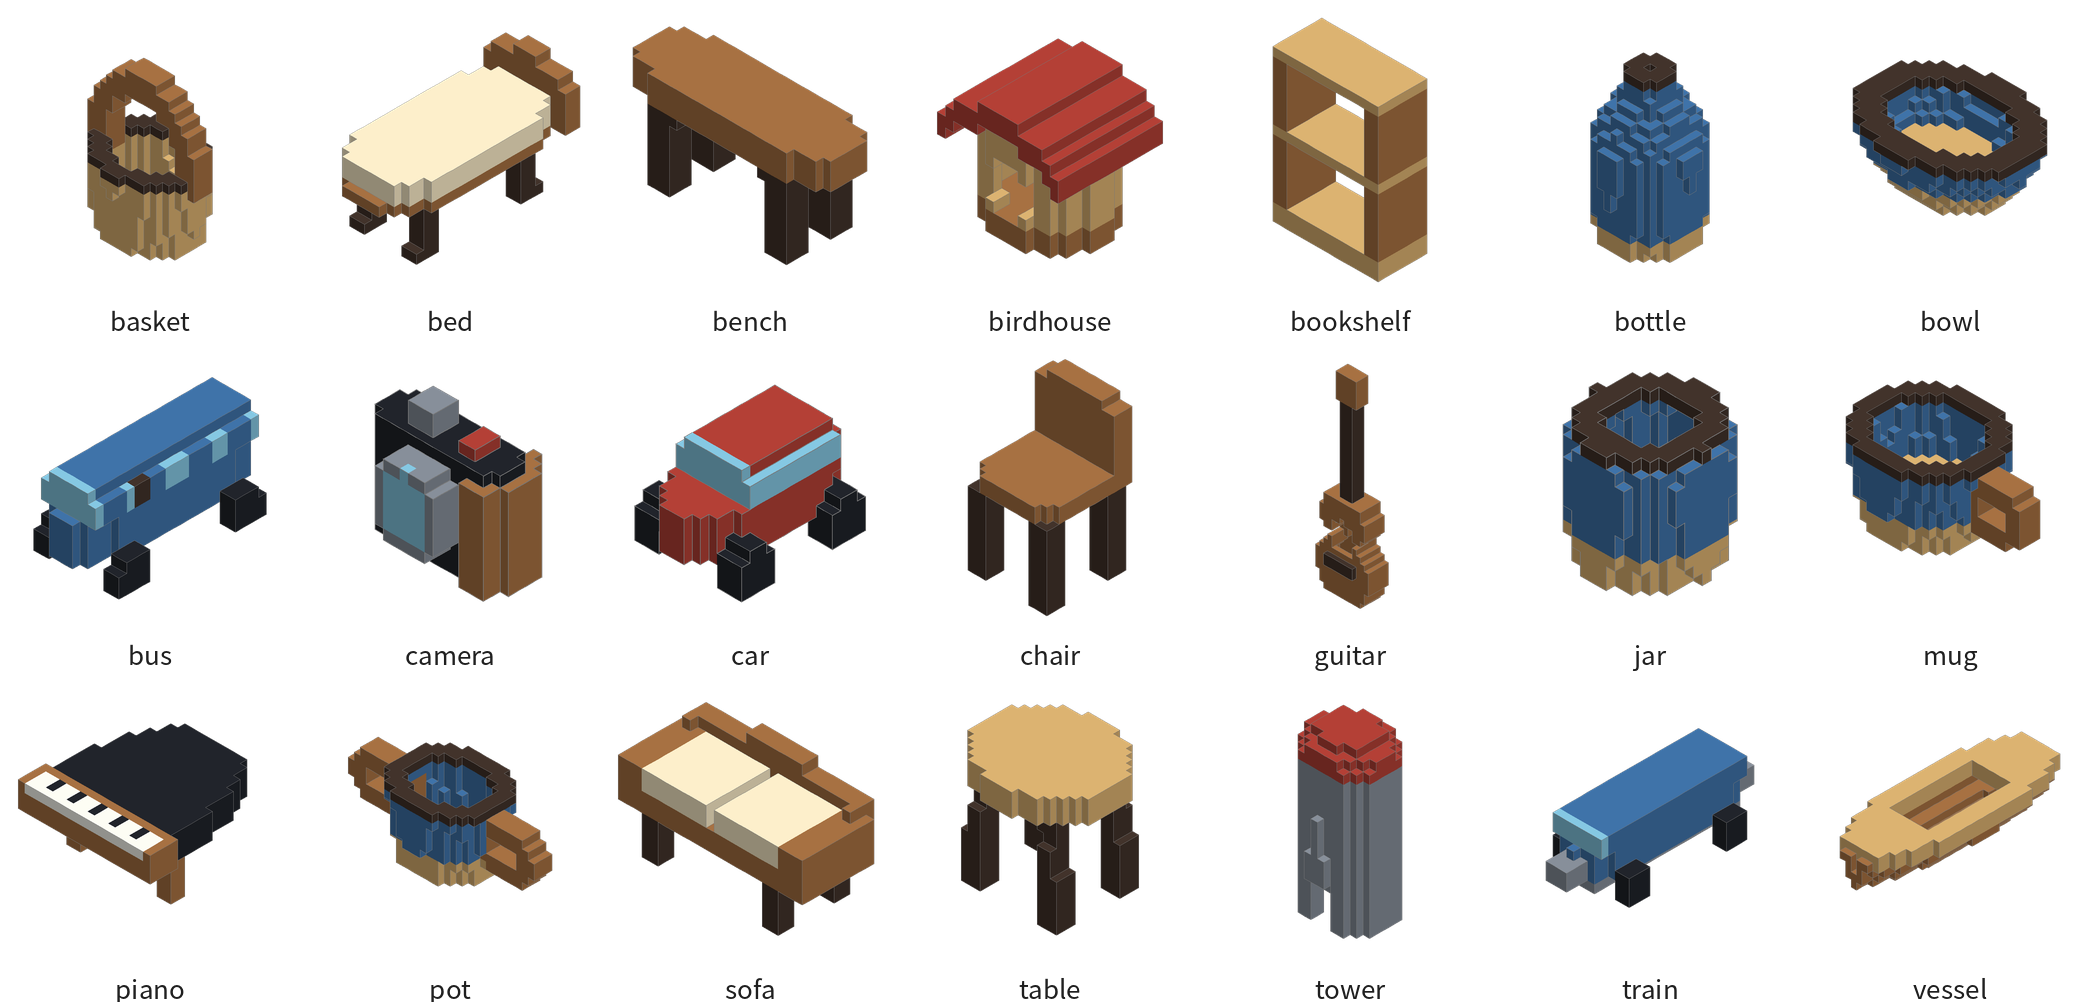
\includegraphics[width=0.475\textwidth]{figures/image7.png}\hfill
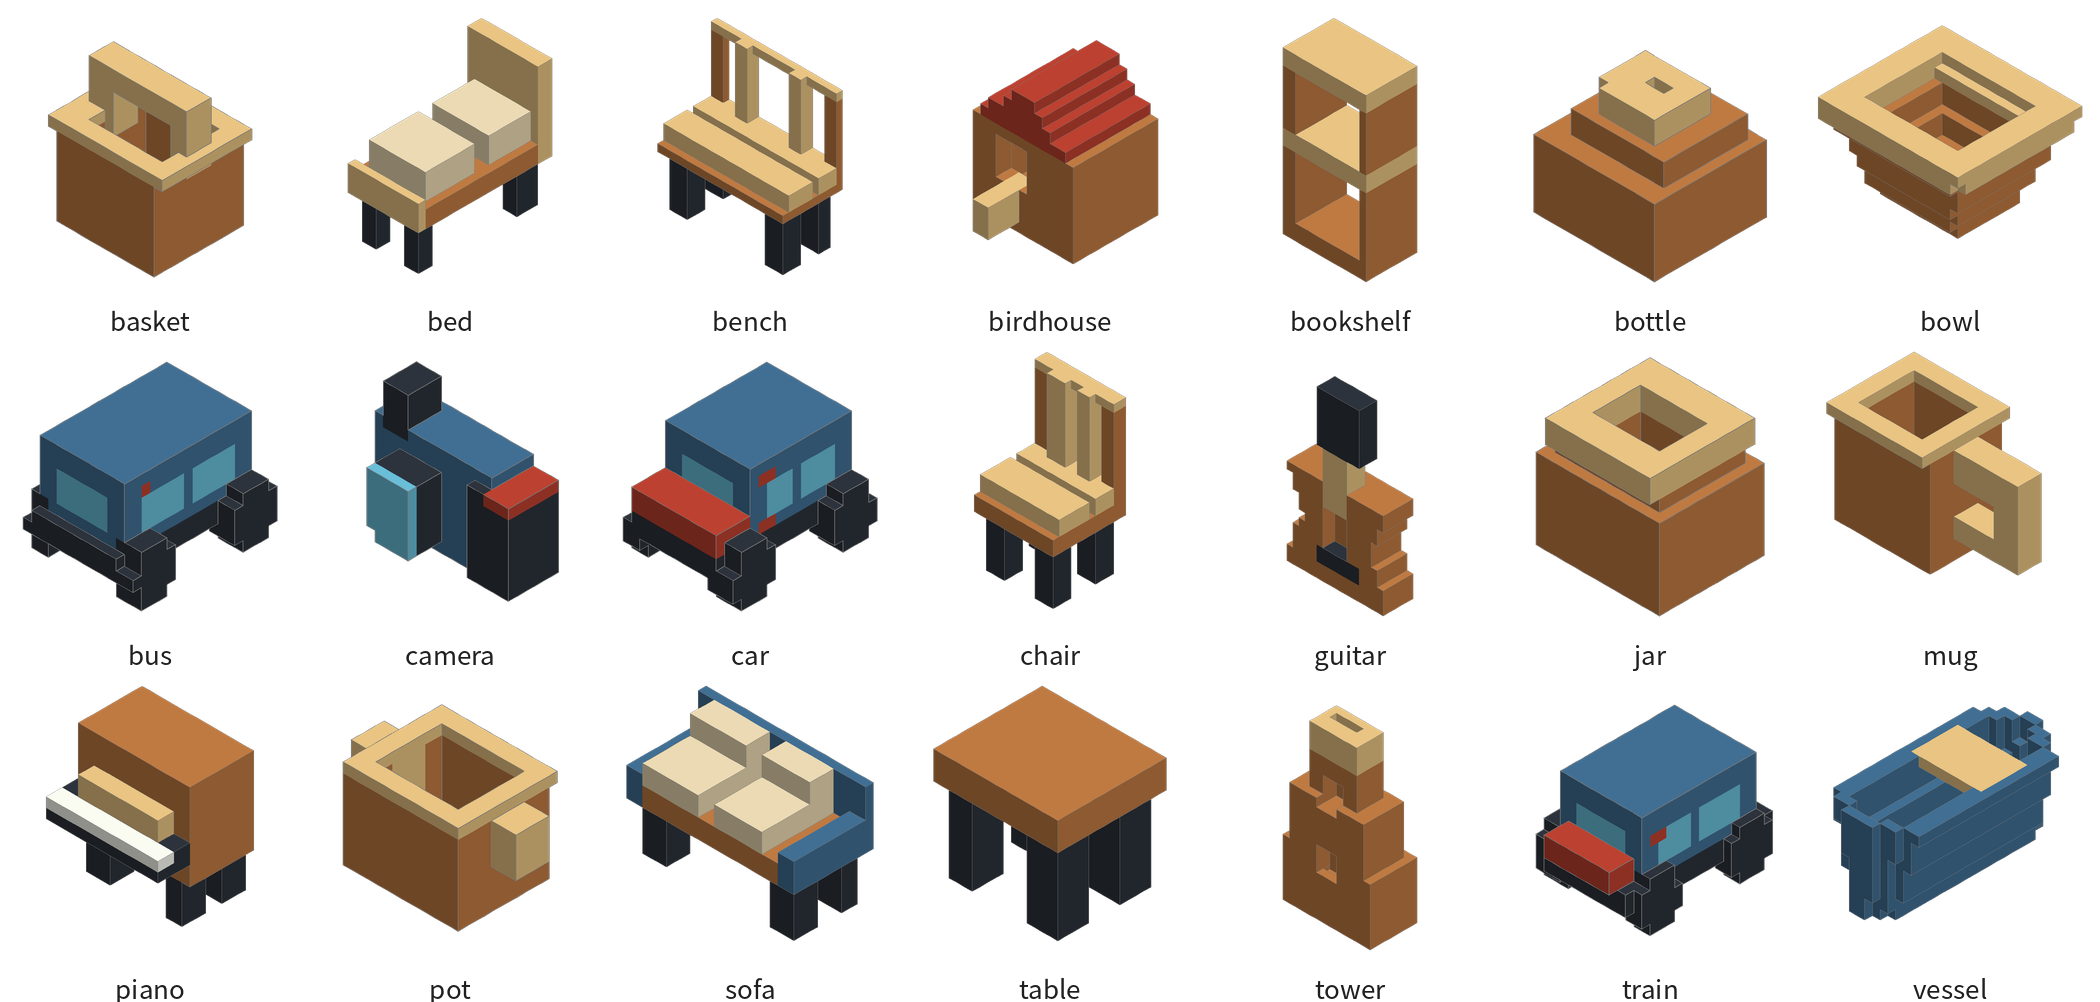
\includegraphics[width=0.475\textwidth]{figures/image8.png}
\caption{Voxel model samples spanning the 21 object categories.}
\end{figure*}

\begin{figure*}[!htbp]
\centering
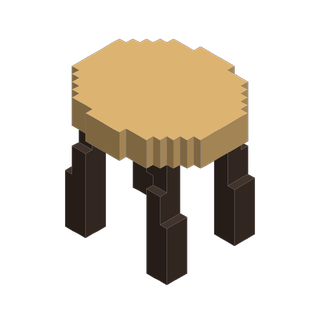
\includegraphics[width=0.118\textwidth]{figures/image4.png}\hfill
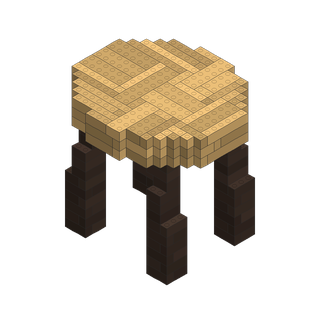
\includegraphics[width=0.118\textwidth]{figures/image5.png}\hfill
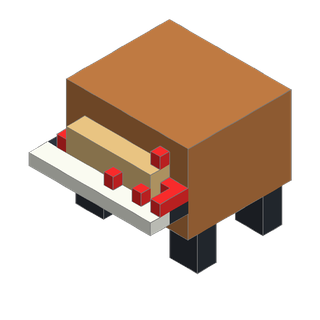
\includegraphics[width=0.118\textwidth]{figures/image2.png}\hfill
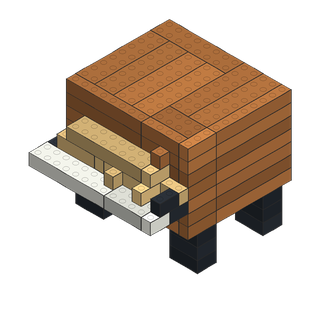
\includegraphics[width=0.118\textwidth]{figures/image3.png}\hfill
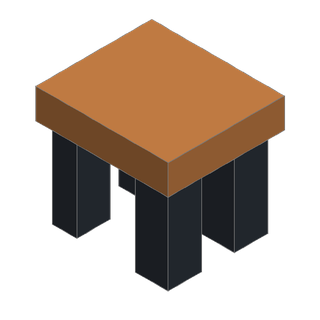
\includegraphics[width=0.118\textwidth]{figures/image9.png}\hfill
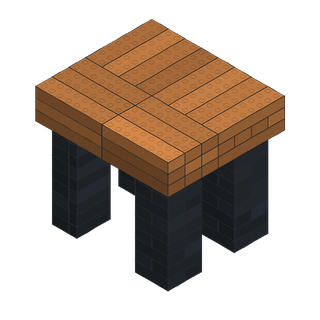
\includegraphics[width=0.118\textwidth]{figures/image10.png}\hfill
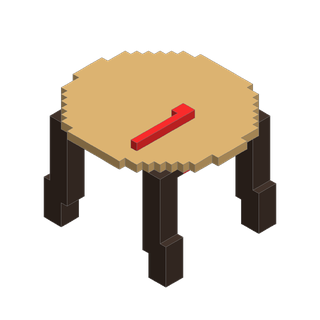
\includegraphics[width=0.118\textwidth]{figures/image11.png}\hfill
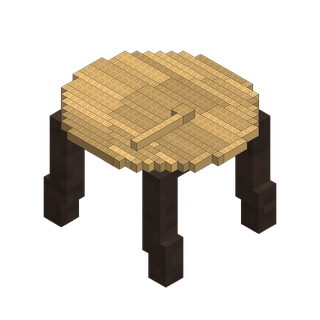
\includegraphics[width=0.118\textwidth]{figures/image12.png}
\caption{Historical examples of voxel targets and brick layouts after local repair.}
\end{figure*}

\begin{figure}[!htbp]
\centering
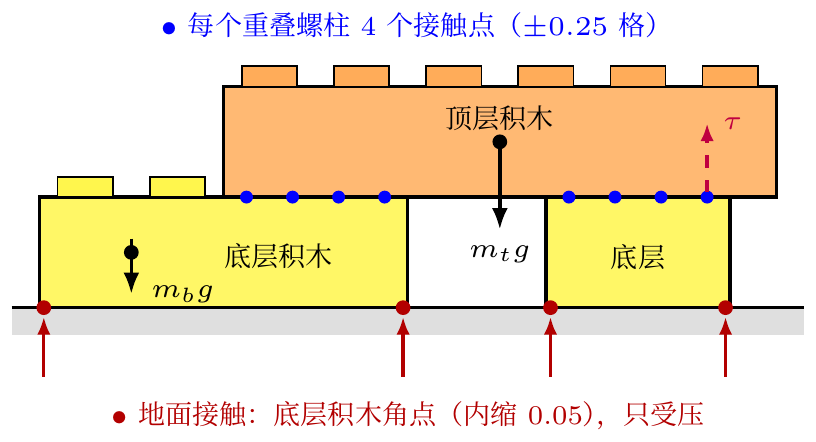
\includegraphics[width=\columnwidth]{figures/image13.png}
\caption{Historical contact-based gravity screening model (source labels in Chinese are retained).}
\end{figure}

\begin{figure*}[!htbp]
\centering
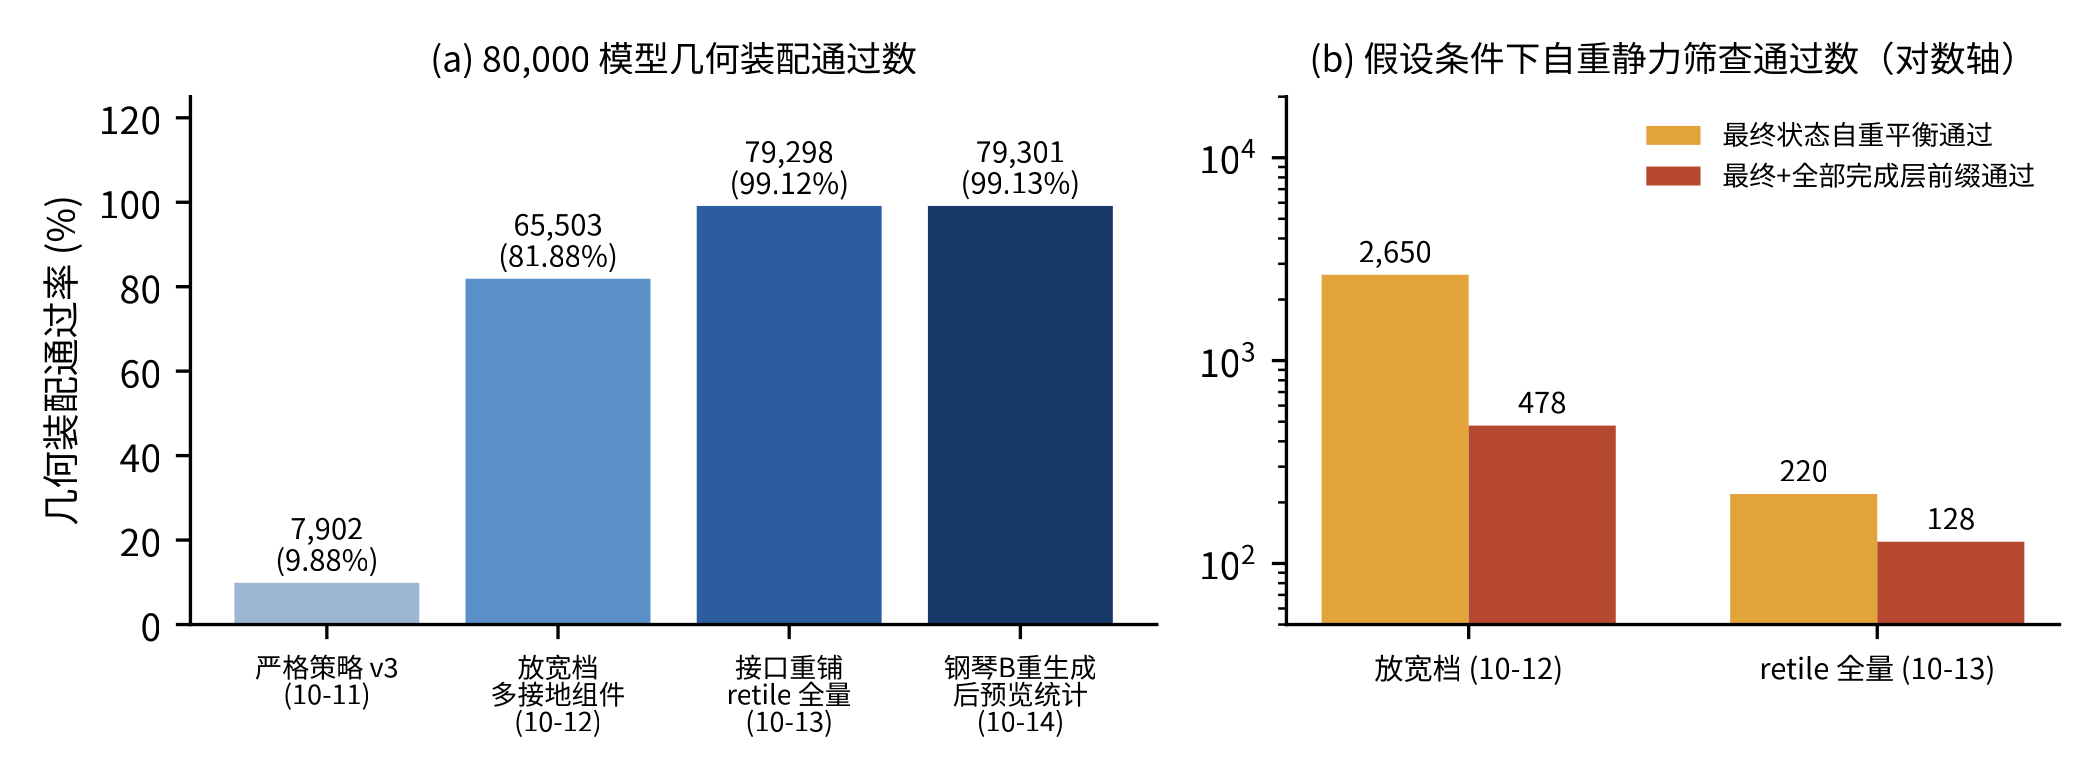
\includegraphics[width=0.85\textwidth]{figures/image14.png}
\caption{Historical comparison of geometric conversion and screening outcomes across releases. Version and numerical labels require verification.}
\end{figure*}

\begin{figure*}[!htbp]
\centering
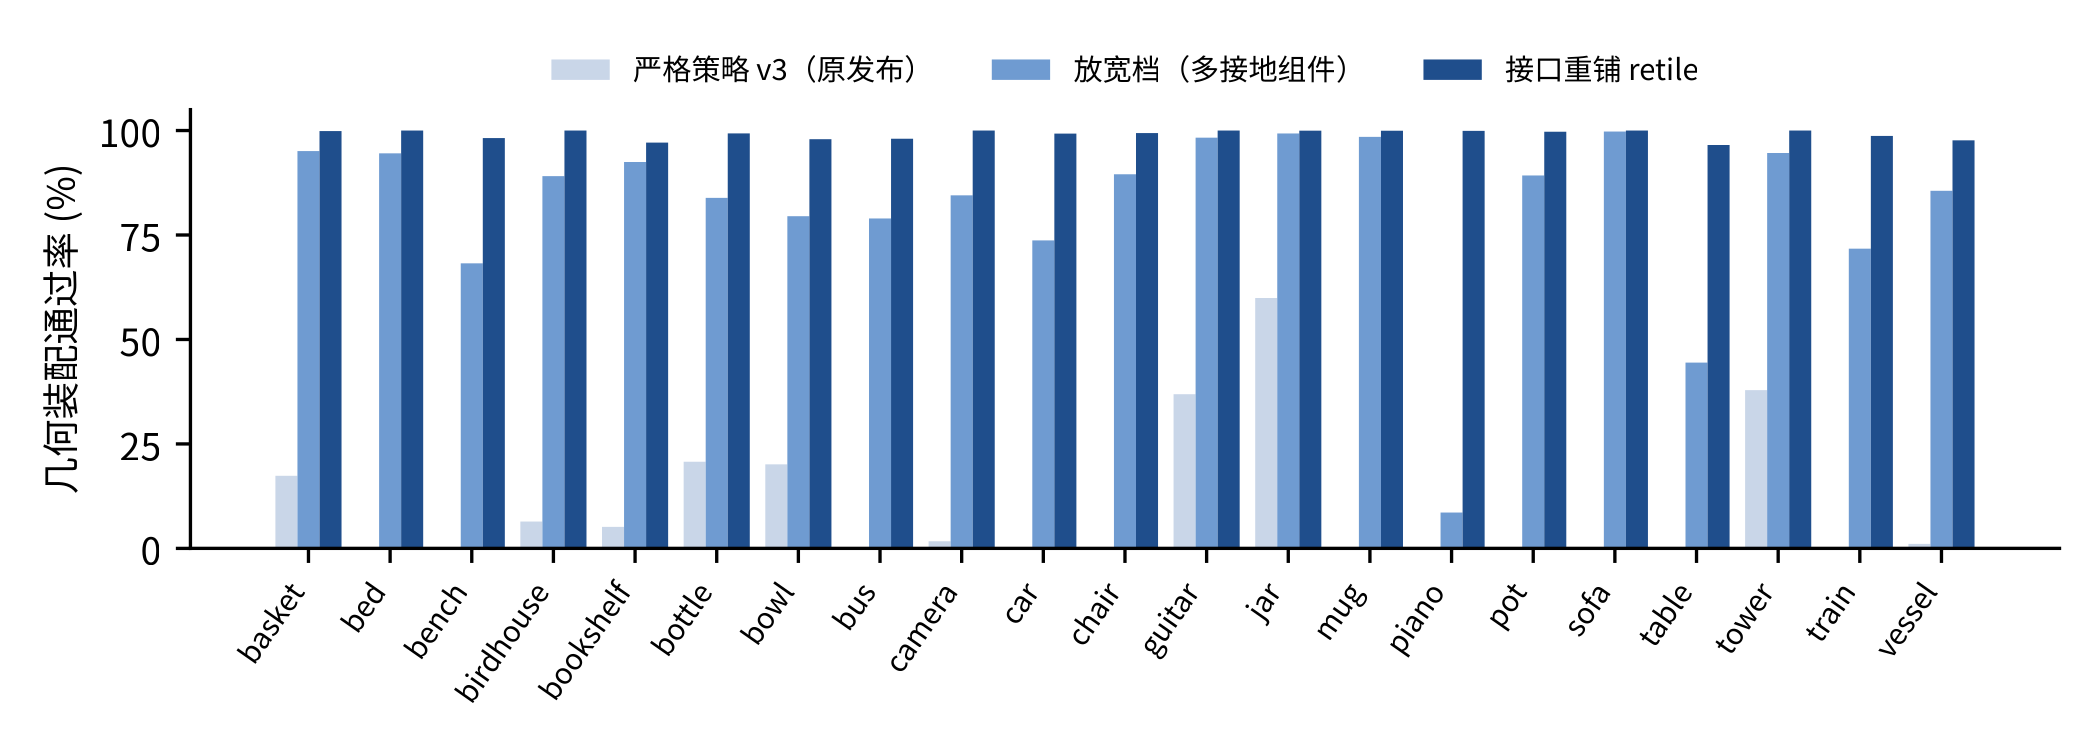
\includegraphics[width=0.85\textwidth]{figures/image15.png}
\caption{Historical category-level geometric pass rates. Version and numerical labels require verification.}
\end{figure*}

\begin{figure}[!htbp]
\centering
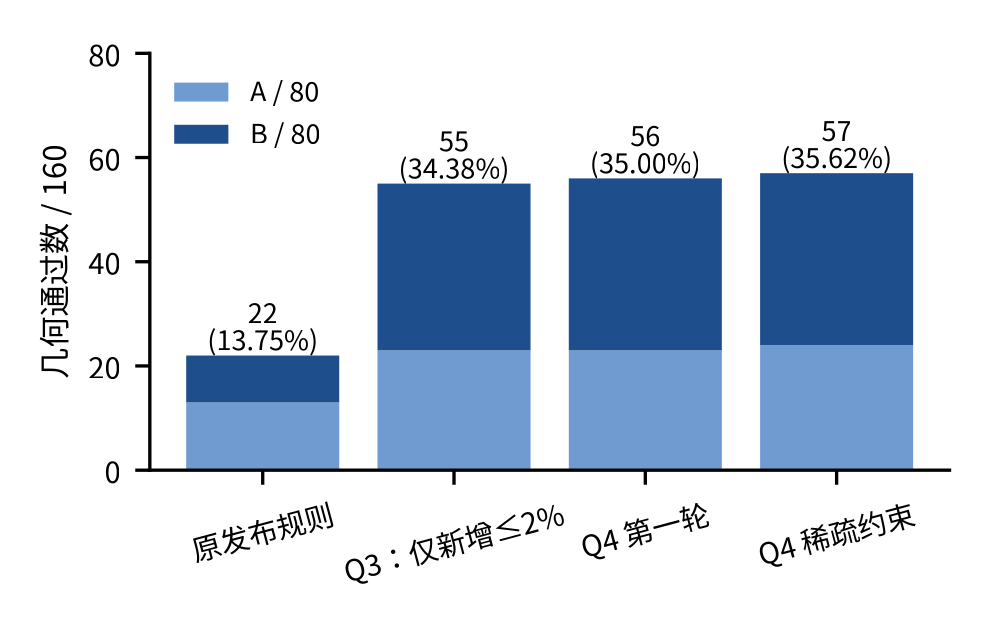
\includegraphics[width=\columnwidth]{figures/image16.png}
\caption{Historical results on a uniform 160-model sample. Version and numerical labels require verification.}
\end{figure}

\begin{figure*}[!htbp]
\centering
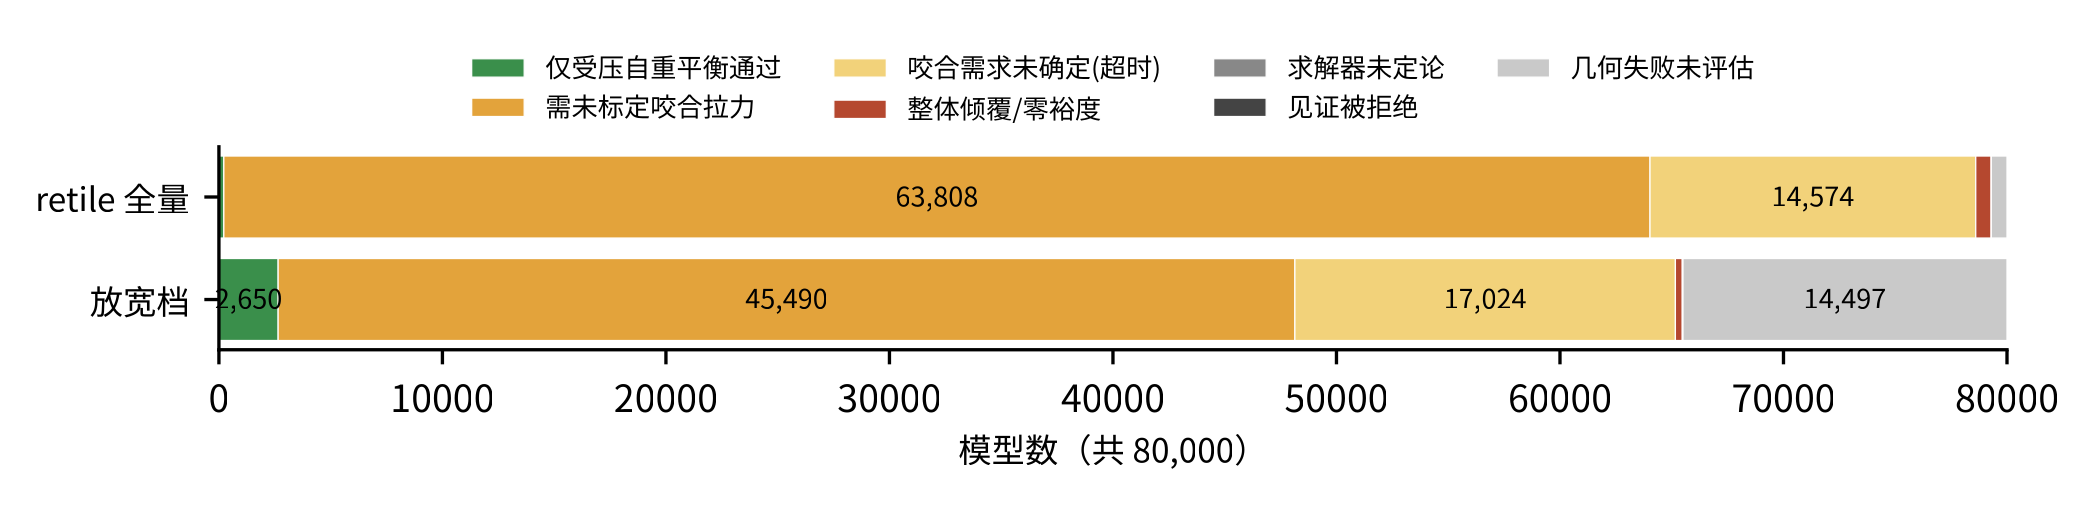
\includegraphics[width=0.85\textwidth]{figures/image17.png}
\caption{Historical distributions of physical screening statuses. Counts refer to the specific releases shown and are kept separate from geometric pass rates.}
\end{figure*}

\FloatBarrier
\section{Technical Appendix: Training Details}
\label{app:training}
Aggregate throughput is 24,448 tokens/s over eight GPUs, and the mean training loss is 0.0273. Evaluation and checkpointing run every 500 steps. With TRL~0.15, the unpacked multi-GPU path hangs after the first backward pass, which is why the TRL~0.17 stack is pinned. Because validation loss is lowest during epoch 2, two epochs would be a more economical setting for future runs (about one third less compute). The full software stack is transformers 4.51.3, trl 0.17.0, peft 0.15.2, datasets 3.6.0, and accelerate 1.6.0, with bf16 precision, gradient checkpointing, and unpacked sequences.

\begin{table}[!htbp]
\centering
\small
\begin{tabular}{lrr}
\toprule
Progress & Step & Validation loss \\
\midrule
Start & 500 & 0.1410 \\
--- & 1,500 & 0.0950 \\
--- & 10,500 & 0.0509 \\
--- & 22,500 & 0.0404 \\
$\approx$ End of epoch 1 & 44,500 & 0.0337 \\
--- & 65,500 & 0.0316 \\
Best (epoch 1.77) & 79,000 & 0.0308 \\
End of epoch 3 & 133,860 & 0.0339 \\
\bottomrule
\end{tabular}
\caption{Validation loss on the 2,000-sample validation subset. One epoch is $\approx$44,620 steps; the nearest evaluation to the end of epoch 1 is step 44,500.}
\label{tab:eval-loss}
\end{table}

% BrickGPT-paper column verified against arXiv:2505.05469 (Sec. 5.1 and Appendix A training details).
\begin{table*}[!htbp]
\centering
\small
\setlength{\tabcolsep}{5pt}
\begin{tabular}{lcc}
\toprule
Dimension & BrickGPT paper & Official Qwen3 script (ours) \\
\midrule
Base model & LLaMA-3.2-1B-Instruct & Qwen3-1.7B \\
LoRA & $r=32$, $\alpha=16$, dropout $0.05$, $q$/$v$ only (3.4M params) & $r=16$, $\alpha=32$, all linear layers \\
Learning rate & $2{\times}10^{-3}$ (AdamW) & $10^{-4}$ \\
Effective batch & 64 & 8 \\
Max length & 4,096 & 8,192 \\
Epochs & 3 & 3 \\
Hardware & 8$\times$RTX A6000, 12\,h & 8$\times$4090D, 25.3\,h \\
Data & StableText2Brick, 47k structures / 240k prompts & BrickMore-48, 79.3k models / 396,610 samples \\
\bottomrule
\end{tabular}
\caption{Our configuration versus the original BrickGPT paper \cite{brickgpt}. BrickGPT-paper values are taken from Sec.~5.1 and Appendix~A of arXiv:2505.05469 (base model, LoRA $r{=}32$, $\alpha{=}16$, dropout $0.05$, $q$/$v$ only with 3.4M parameters, AdamW learning rate $0.002$, global batch 64, 4096-token length filter, 3 epochs, 8$\times$RTX A6000 and 12\,h, and 47k+ structures / 240k prompts). The data organization, instruction template, absence of thinking mode, and LoRA paradigm follow BrickGPT; concrete hyperparameters follow the official Qwen3 adaptation, with the budget adjusted for the larger world, library, and corpus.}
\label{tab:brickgpt-recipe}
\end{table*}

\FloatBarrier
\section{Technical Appendix: Additional Evaluation Material}
\label{app:eval}

\begin{figure*}[!htbp]
\centering
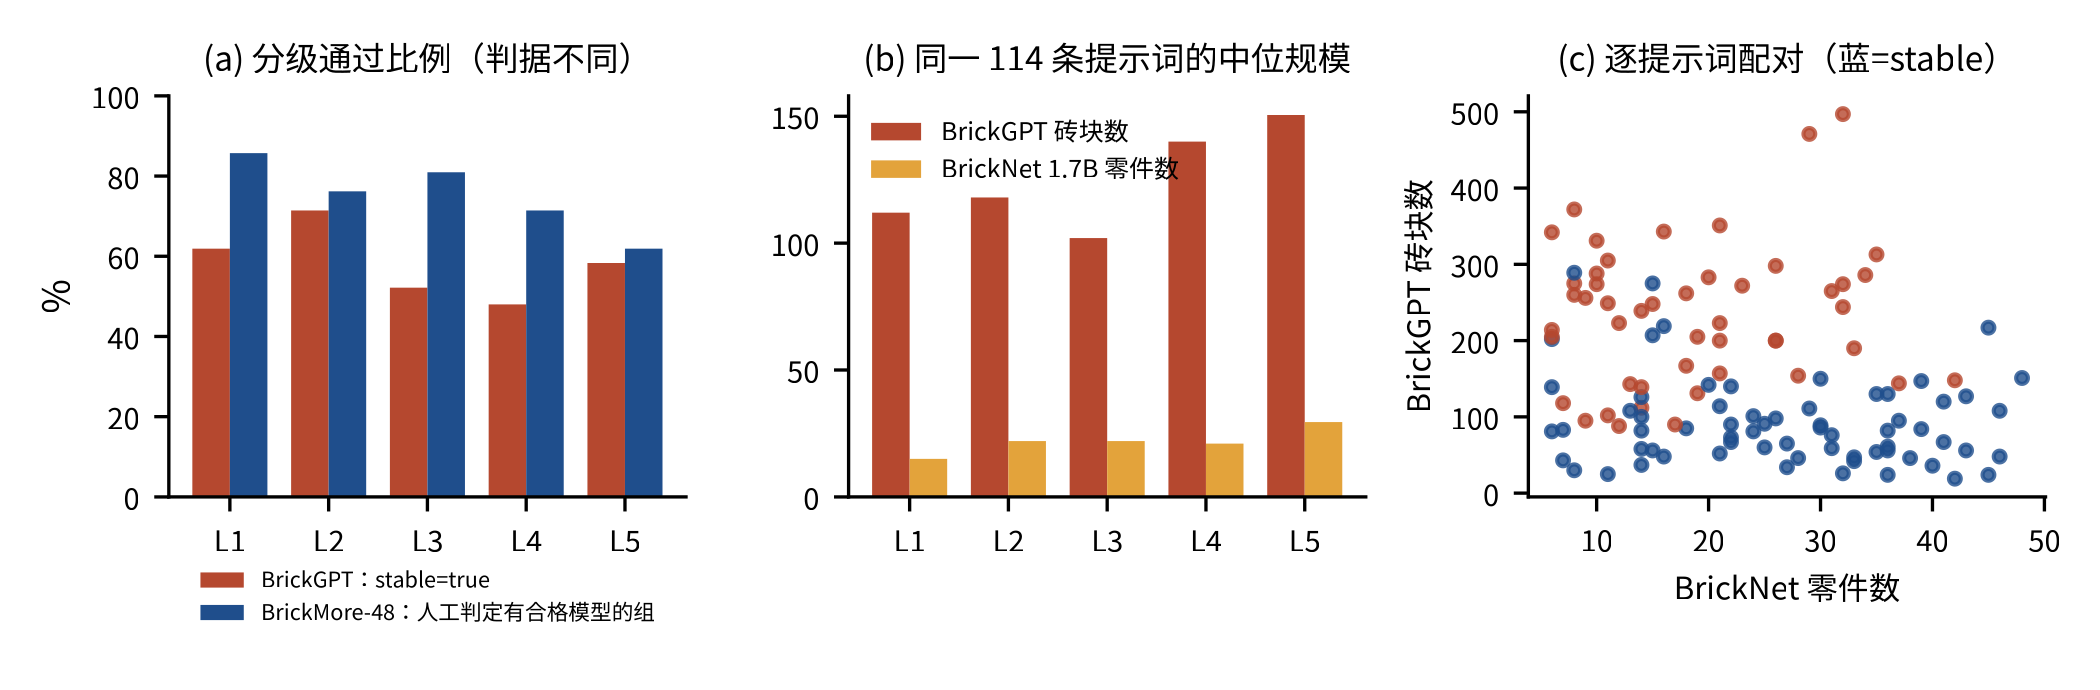
\includegraphics[width=0.85\textwidth]{figures/image18.png}
\caption{Historical baseline comparison with differing acceptance criteria; not the current matched main comparison.}
\end{figure*}

\begin{figure*}[!htbp]
\centering
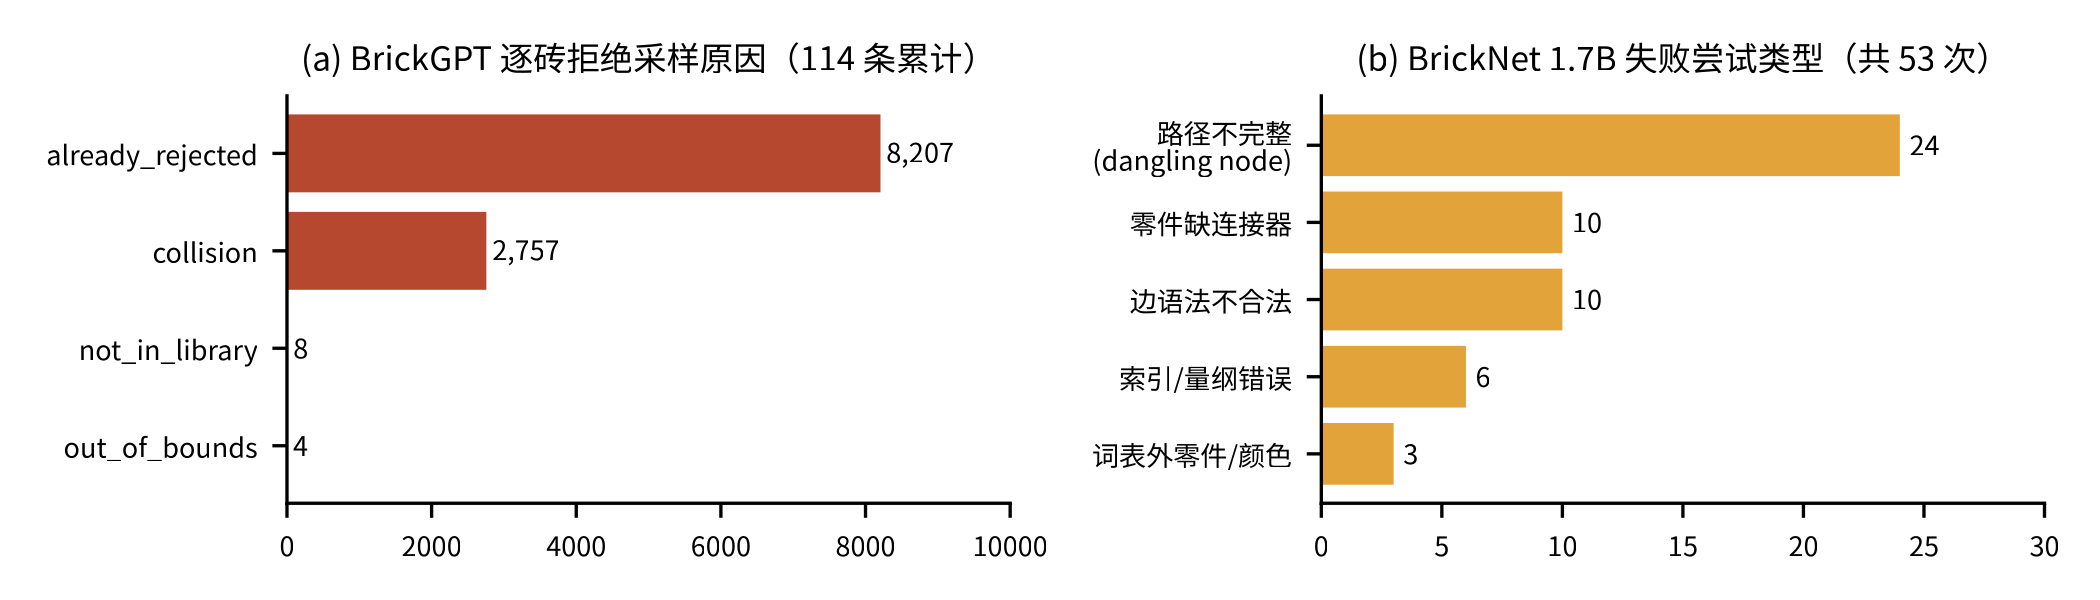
\includegraphics[width=0.85\textwidth]{figures/image19.png}
\caption{Historical failure categories in the supplied reference; sample definitions require verification.}
\end{figure*}

\begin{figure*}[!htbp]
\centering
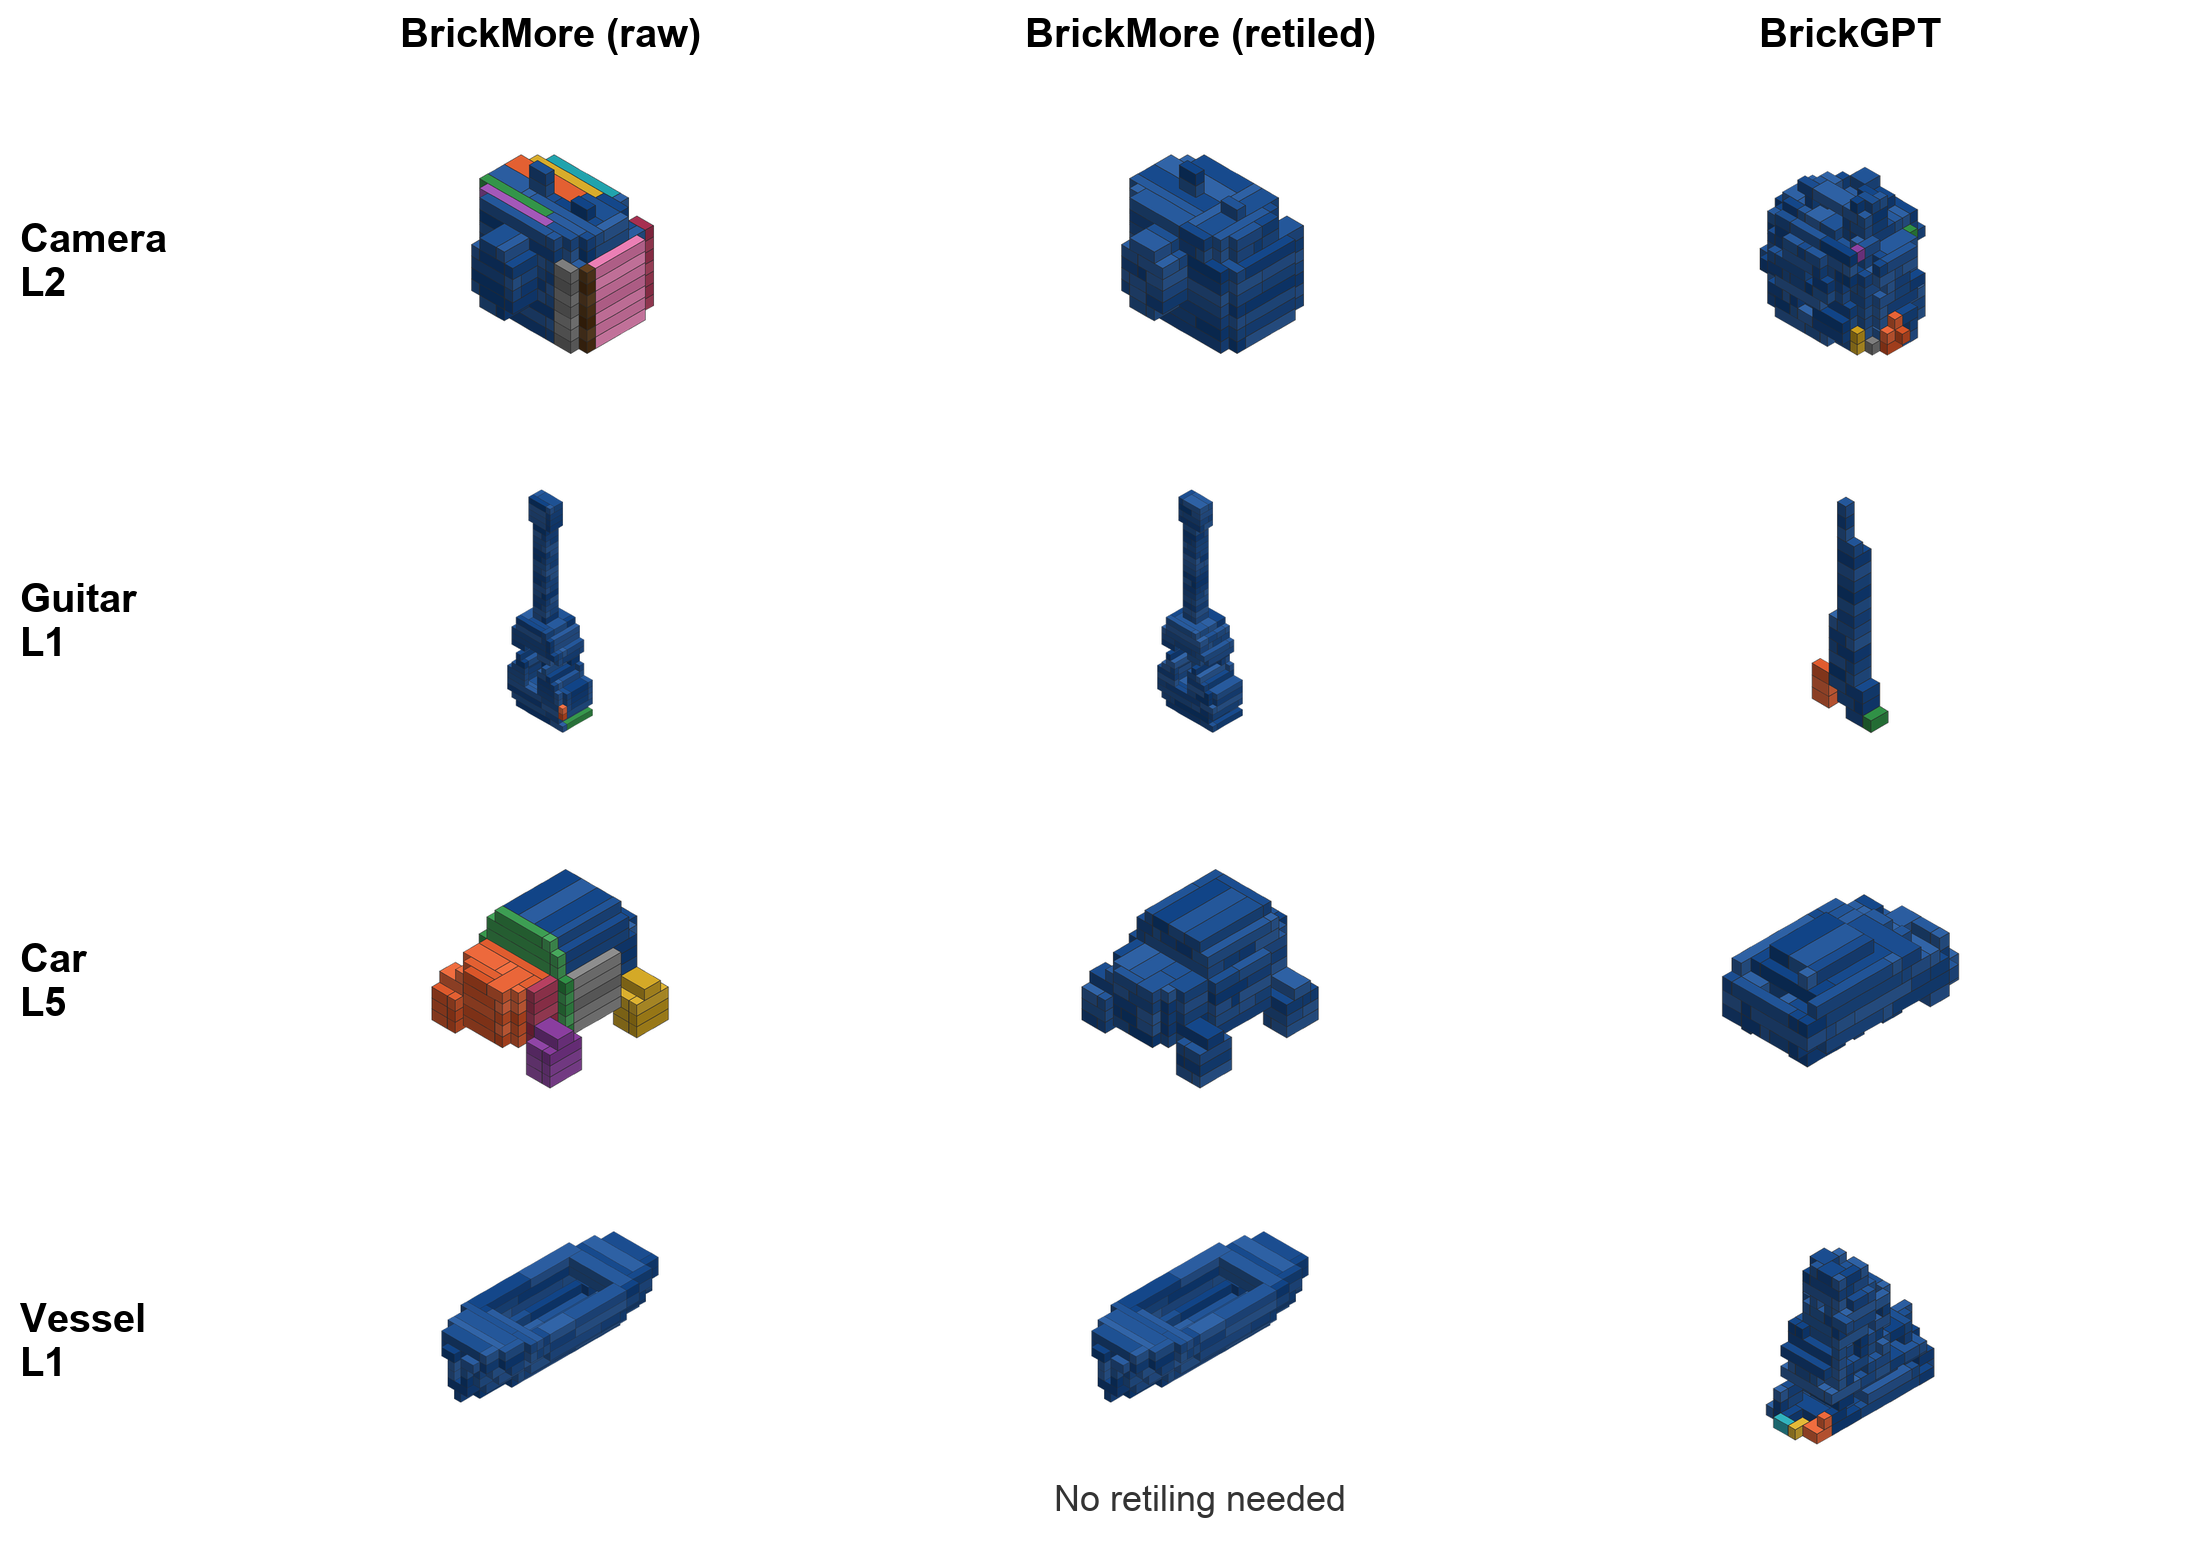
\includegraphics[width=0.85\textwidth]{figures/original_comparison.png}
\caption{Qualitative historical examples from the supplied reference. Column labels distinguish raw BrickMore, retiled BrickMore, and BrickGPT outputs.}
\end{figure*}

\FloatBarrier
\section{Technical Appendix: Historical Tables}
\label{app:historical}
The following transcribed tables preserve the historical reference material. They use different versions or evaluation criteria and are not substitutes for the current main comparison. Dashes indicate missing entries in the supplied source.
\begin{table*}[!htbp]\centering\small
\begin{tabular}{lr}\toprule
Item & Historical value \\ \midrule
Voxel models & 80,000 (40,000 per batch) \\
Categories / structural families & 21 / 40 per category \\
Grid / voxel count & $48^3$ / 750--1,250 \\
Prompt records & 400,000 (five bilingual records per model) \\
Uniqueness & 80,000 unique; 0 A/B duplicates \\
Overlap with historical hashes & 0 / 55,255 \\
Retile geometry passes & 79,298 (99.12\%) \\
Bricks in full preview & 12,718,389 \\
Final gravity equilibrium passes & 220 \\
Final and layer-prefix passes & 128 \\
\bottomrule\end{tabular}
\caption{Historical dataset statistics transcribed from the supplied reference. The geometry count refers to the old retile release, not the later integrated count. Verify the preview and physical-screening totals against version-matched reports.}
\end{table*}

\begin{table*}[!htbp]\centering\scriptsize
\begin{tabular}{llrrrrr}\toprule
Version & Connectivity & Voxel changes & Passes & Rate & Final & Final + prefixes \\ \midrule
Strict v3 & Single; support $\geq$10\%, overhang $\leq$2 & None & 7,902 & 9.88\% & -- & -- \\
Relaxed & Each component grounded & +428,278 / -38,230 & 65,503 & 81.88\% & 2,650 & 478 \\
Retile & Each component grounded & +228,582 / -125 & 79,298 & 99.12\% & 220 & 128 \\
\midrule
\multicolumn{7}{l}{Uniform 160-model sample (seed 38177); not full-dataset results} \\
Baseline & Single stud-connected component & None & 22 & 13.75\% & -- & -- \\
Q3 & Single stud-connected component & Added $\leq$2\% & 55 & 34.38\% & 8 & 2 \\
Q4 (sparse) & Single stud-connected component & Added + removed $\leq$2\% & 57 & 35.63\% & 8 & 2 \\
\bottomrule\end{tabular}
\caption{Historical conversion-strategy table from the reference. Full-dataset and 160-model sample rows use different scopes; connectivity rules also differ. Final and prefix columns report screening outcomes under the stated historical assumptions.}
\end{table*}

\begin{table*}[!htbp]\centering\small
\begin{tabular}{lrrr}\toprule
Item & BrickGPT & BrickNet 1.7B & BrickMore-48 \\ \midrule
Representation & $20^3$ bricks & Assembly graph & $48^3$ bricks \\
Criterion & stable & Parseable & -- \\
Passes & 66/114 & 114/114 & -- \\
Median parts & 126.5 & 22 & -- \\
Range & 19--497 & 6--48 & -- \\
Mean time (s) & 189.6 & -- & -- \\
\bottomrule\end{tabular}
\caption{Historical baseline table in the source reference. These criteria differ, and missing BrickMore entries were marked TODO. This is not the current matched four-metric main table.}
\end{table*}

\begin{table*}[!htbp]\centering\small
\begin{tabular}{lrrrrl}\toprule
Level & $n$ & BrickGPT stable & BrickGPT median bricks & BrickNet median parts & BrickMore-48 \\ \midrule
L1 & 21 & 13 & 112 & 15 & -- \\
L2 & 21 & 15 & 118 & 22 & -- \\
L3 & 23 & 12 & 102 & 22 & -- \\
L4 & 25 & 12 & 140 & 21 & -- \\
L5 & 24 & 14 & 150.5 & 29.5 & -- \\
\bottomrule\end{tabular}
\caption{Historical level-wise baseline table transcribed from the reference. The original BrickMore column was incomplete, and the other columns use different criteria.}
\end{table*}

\begin{table*}[!htbp]\centering\small
\begin{tabular}{lrrrr}\toprule
Method and source & $P_{\mathrm{inv}}$ & VQA & PE & SigLIP2 \\ \midrule
BrickGPT (literature, as transcribed) & 0.063 & 0.050 & 0.157 & 0.052 \\
BrickNet 1.7B (literature, as transcribed) & 0.260 & 0.593 & 0.282 & 0.631 \\
BrickGPT (114 prompts, historical placeholder) & -- & -- & -- & -- \\
BrickNet (114 prompts, historical placeholder) & -- & -- & -- & -- \\
BrickMore-48 (114 prompts, historical placeholder) & -- & -- & -- & -- \\
\bottomrule\end{tabular}
\caption{Original reference table with literature values and historical placeholders. Literature values use another evaluation set and must not be directly compared with the present 114-prompt results; the precise $P_{\mathrm{inv}}$ definition and direction require checking against the original publication.}
\end{table*}


\FloatBarrier
\end{document}
